\documentclass[12pt]{article}
\usepackage{titlesec}
\usepackage{setspace}
\usepackage{graphicx} 
\usepackage{color}
\usepackage{hyperref}
\usepackage{amsmath}
\usepackage[left=1.5in,top=1in,right=1in,bottom=1in]{geometry}
\textwidth 6in
\textheight 9in
\parskip 7.2pt           % sets spacing between paragraphs
\parindent 0pt		 % sets leading space for paragraphs
\titleformat{\section}{\bfseries}{\thesection}{12pt}{}
\newcommand{\sectionbreak}{\clearpage}
\begin{document}         
% Start your text

%\color{blue}

\begin{center}
\break \break \break \break 

%The Plasticity and Generalizability of Deep Networks
%The Adaptability of Stacked Denoising Autoencoders
Learning General Features From Images and Audio With Stacked Denoising Autoencoders.
\break\break\break\break \break \break \break \break \break 
by \break \break Nathan H. Nifong
\break\break\break\break \break \break \break \break \break 
A thesis submitted in partial fulfillment of the\break
requirements for the degree of
\break\break\break\break 
Master of Science \break in \break Systems Science
\break\break\break\break \break 
Thesis Committee: \break Wayne Wakeland, \break Marty Zwick, \break Melanie Mitchell.
\break\break\break\break 
Portland State University \break 2013
\end{center}

\begin{singlespacing}
\tableofcontents
\end{singlespacing}

\section*{Abstract}
\label{Abstract}
\begin{doublespacing}

One of the most impressive qualities of the brain is its neuro-plasticity. The neocortex has roughly the same structure throughout its whole surface, yet it is involved in a variety of different tasks from vision to motor control, and regions which once performed one task can learn to perform another \cite{hawkins2004intelligence}. Machine learning algorithms which aim to be plausible models of the neocortex should also display this plasticity. One such candidate is the stacked denoising autoencoder (SDA). SDA's have shown promising results in the field of machine perception where they have been used to learn abstract features from unlabeled data. \cite{larochelle2007empirical, le2011building, vincent2008extracting} In this thesis I develop a flexible distributed implementation of an SDA and train it on images and audio spectrograms to experimentally determine properties comparable to neuro-plasticity, Specifically, I compare the visual-auditory generalization between a multi-level denoising autoencoder trained with greedy, layer-wise pre-training (GLWPT), to one trained without. I test a hypothesis that networks pre-trained on one sensory modality will perform better on the other modality than randomly initialized networks trained for an equal total number of epochs. Furthermore, I also test the hypothesis that the magnitude of improvement gained from this pre-training is greater when GLWPT is applied than when it is not.

\section{Introduction and Background}

	\subsection{Introduction}
		It is an ongoing effort in machine learning to match the powerful learning capacity of the human brain. Deep belief networks are a recently successful neurally inspired class of machine learning algorithms. In this thesis I set out to investigate the plasticity, or adaptability, of stacked denoising autoencoders, a type of deep belief network. See section 2.6 and figure~\ref{fig:sda_struct} for an explanation of SDA's. Plasticity gives us an idea of how brain-like the SDA algorithm is. If we seek to make brain-like learning algorithms, using the "intelligence" of those algorithms as a measure of success is both too vague, and too distant to be useful. If we instead look for esoteric behaviors and qualities that we know to be brain-like, such as plasticity, it reveals more readily applicable clues about where to invest our efforts in further research\cite{hinton1995wake}.
		Following from this motive I measure the plasticity of SDA's by switching models between data from two different sensory modalities, images and audio, and observing the effect on reconstruction accuracy. I test two distinct hypotheses:
\begin{enumerate}
	\item SDA models trained on one sensory modality and then switched to a second sensory modality half-way through training will have a higher reconstruction accuracy on test data from the second sensory modality than randomly initialized networks trained for an equal total number of epochs on the second sensory modality exclusively.
	\item When hypothesis 1 is tested using SDA's trained with greedy layer-wise pre-training vs. SDA's without, the magnitude of the difference in reconstruction accuracy described in hypothesis 1 will be greater for SDA's trained with greedy layer-wise pre-training.
\end{enumerate}
		The hypotheses are tested by training stacked denoising autoencoders on an image dataset and an audio dataset with identical dimensionalities. Three variables are manipulated: single or multi-modal training data, layer-wise or interleaved layer training order, and audio or images as the test data. There are 8 experiments in total, each one run with 20 different random seeds.
		In conclusion I found that GLWPT helped the SDAs learn abstract features, but this did not help it's cross-modal generalization. I address the unexpected differences between models tested on audio vs. images, and discuss potential causes and fixes. I include visualizations of the features learned and graphs of the reconstruction error over time for each layer in several pairs of models. These figures illustrate interesting unexpected observations about the training process which could be the focus of future work.

	\subsection{Neural Plausibility of Machine Learning Algorithms}
		The latest strides in the field of machine learning are coming from deep networks \cite{bengio2009learning, grubb2010boosted, hinton2012deep, lee2009convolutional, krizhevsky2012imagenet, tang2012deep}. This class of learning algorithm is inspired by the structure of the mammalian neocortex, specifically the visual areas in the occipital lobe which have been studied more extensively than any other part. This is in contrast to non-neurally inspired algorithms such as support vector machines  (SVM) that are more widely used and were notably better at classification than neural networks\cite{byvatov2003comparison, ding2001multi, mukkamala2002intrusion}. Now that we are seeing biologically inspired algorithms leading the way, biological plausibility becomes a useful heuristic for the further development of algorithms with higher performance measures, and discoveries about the emergent properties of these algorithms may feed back into neuroscience to inform further study of the brain. 
		One metric which defines the brain and differentiates it from other intelligent systems is its plasticity. Areas which once specialized in a certain function can change and learn a new function if for some reason they cannot continue with their first function or if the second function is just much more demanding of computational resources. \cite{sharma2000induction}
		
	\subsection{Hierarchical representation in the brain}
		Deep networks are like the neocortex in many ways, but the most important of them is the hierarchical structure from which they get their name. In the visual cortex, neuroscientists have found using single-neuron recording that there are cells which respond most strongly to specific visual stimuli. The nature of the stimuli which excite the neurons changes changes along many dimensions throughout the visual cortex. One of the more salient dimensions of variation is that of \em abstraction\em\cite{hinton2005kind}. The organization of the visual cortex is illustrated in figure ~\ref{fig:visualcortex}. The cells in V1 are the first cells in the cortex to receive signals from the retina via the lateral genticulate nucleus, a part of the thalamus. Cells here respond most actively to a particular edge at a particular angle within a small area of vision called their receptive field. As one moves up V2, V3, V4, and V5 the cells respond to more and more abstract visual stimuli until one sees cells that do things like activating whenever a dog is in the visual field, when objects appear to be moving in a specific way, and even abstract visual conditions such as "currently looking at object in hand" regardless of what or where it is. While it is possible that each of those abstract stimuli has a large set of neurons dedicated to recognizing it out of a "raw" sensory stream, it's far more plausible that they recognize it out of a small, and information-rich stream of intermediate representations. This leads to the idea that a hierarchical structure is crucial to the functionality of the neocortex.
		% cite something about how the brain's plasticity is thanks to abstraction and generalization, and not an ability to "erase and start over"
		
\begin{figure}[p]
\centering
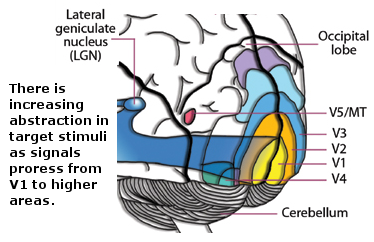
\includegraphics[scale=0.8]{visual_cortex}
\caption{An illustration of the areas within the visual cortex. The layers in a deep networks mimic the stages of processing in the visual cortex. From \em On The Origin Of The Human Mind \em by Andrey Vyshedskiy \cite{vyshedskiy2008origin}}
\label{fig:visualcortex}
\end{figure}

\begin{figure}[p]
\centering
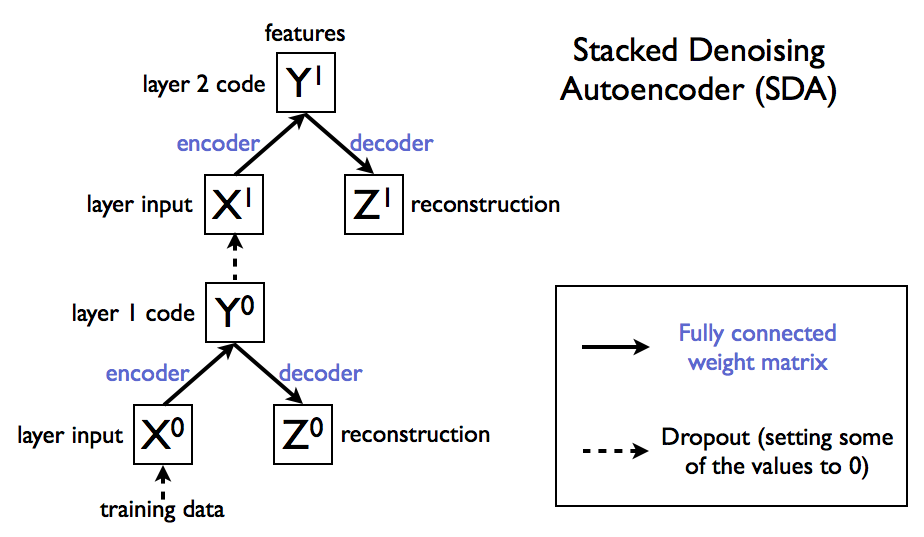
\includegraphics[width=6in]{key1001}  
% Write a better description
\caption{Stacked denoising autoencoder}
\label{fig:sda_struct}
\end{figure}
		
	\subsection{The reusability of hierarchical representations.}
	A hierarchical, or tree-like, structure of knowledge representation allows one to construct compact representations of a massive and complex distribution of stimuli. When building a hierarchy to represent a distribution of stimuli in a layer-wise procedure, first one learns a finite collection of simple patterns corresponding to local, high-frequency (short-term), salient features in sensory signals. Then, one recursively applies that process to the features learned in the first level to construct another set of more abstract features, which are slightly more location, rotation, and scale invariant. In the case of vision, the levels of a hierarchy of representation might be as follows. Images can all be represented as pixel arrays, And pixel arrays can be represented as a collection of overlapping gradients, edges, and spots chosen from a finite set, and colored with a small finite set of colors. (This is the principle behind JPEG compression and appears to be the principal organization of the visual striate cortex.\cite{daugman1980two}) These patches are commonly compared to Gabor filters, depicted in figure~\ref{fig:gaborz}\cite{daugman1988complete, jain1991unsupervised}, and are the most commonly learned set of features in machine vision. As one moves up the chain of abstraction in vision, nearly all combinations of edges and spots seen in natural images can be represented as a hierarchy of things, stuck to the surfaces of bigger things in roughly specified locations, illuminated from a given angle \cite{gluckman2003kurtosis}. Assuming you have a library of hundreds of thousands of things, and the texture of spots, edges, and colors that typically make up their surface, and the ability to calculate shadows, one can decode, or render, this representation into the one below it.

\begin{figure}[p]
\centering
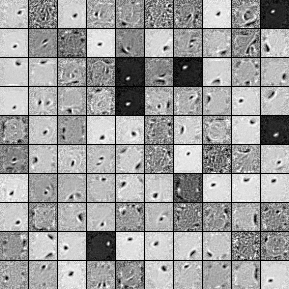
\includegraphics[width=4in,height=4in]{filters_corruption_30}
\caption{Edge, spot and gradient filters learned by a single denoising autoencoder. These are a common and efficient first level feature set for natural images. A feature is actually a set of weights, but an image can be generated to represent it, corresponding to the inputs that would produce a full signal on the given feature, and zero signal on all others. The extent to which these features resemble theoretical Gabor filters is an indicator of how well the model has generalized. This image was generated by me using the same code used in my main experiment. The model was trained on the MNIST digit recognition dataset using a denoising autoencoder.}
\label{fig:gaborz}
\end{figure}
	
	The tricky part of course is learning the vocabularies of symbols that make up each layer and the weights on the connections that allow translation between them. Traditional multi-layer neural networks assume pre-set finite number of layers and nodes at each layer, and then attempt to learn the feed-forward weights which connect layers  all at once using back-propagation and Stochastic Gradient Descent (SGD). There are no weights which operate on the information feeding backwards except in some recurrent neural networks. For the most part, training a multi-layer neural network with only back-propagation and stochastic gradient descent doesn't work very well. On large networks (hundreds of nodes at each layers and more than 3 layers) the search will get stuck in effective local minima\cite{erhan2009difficulty, hinton2006reducing}.
	
	\subsection{Deep networks}
Deep networks can have the same structure as traditional neural networks (set number of layers, set number of nodes at each layer, full feed-forward connections, and sigmoid activation function) but they are trained one layer at a time in order to initialize the optimization procedure for higher layers in a good basin of attraction, and they usually employ some kind of dropout in order to enforce sparse hierarchical representations\cite{hinton2012improving, krizhevsky2012imagenet}. Dropout is a technique of adding noise to data to promote generalizability over accuracy in lower layers. Classical multilayer neural networks must search the entire weight space with no bias or heuristic. For large enough weight spaces, or noisy enough data, Even the best optimization procedure will become trapped in a local minima. Greedy layer-wise pre-training and dropout both help to provide some structure and bias to the search process to reduce the dimensionality of the space, smooth out it's features and discover better minima.  Deep networks have been shown to be able to learn the abstract feature sets that traditional multi-layer neural networks were originally expected to be able to learn\cite{hinton2012deep}. Classical networks can theoretically learn any function, but in practice, they can only learn smooth functions well in a reasonable amount of time. 

There are several types of deep belief networks, but they share the property of having layers stackable interfaces. They consist of a number of modules, which can be increased in depth indefinitely. Denoising autoencoders and Boltzmann machines are commonly used modules\cite{salakhutdinov2007restricted}. The module serves the purpose of performing generalization, and optionally compression. Each module will re-code it's input to a new representation, and this representation serves as the input for the next layer. For each type of module, there are many variants that differ in the method used to learn the parameters, such as marginalized autoencoders, which are optimized for speed \cite{chen2012marginalized}. In order to use a module within a deep network, the module must meet certain criteria. It must perform some limited form of generalization, and must operate on the same format of data it produces, such that it can be stacked recursively. To date, most modules are feed forward only, but several very interesting generative deep recurrent neural networks have also been studied\cite{graves2013generating}.

	\subsection{Stacked denoising autoencoders}
The aim of the autoencoder is to learn the code $\mathbf y$, a distributed representation that captures the coordinates along the main factors of variation in the data, $\mathbf x$ (similar to how principal component analysis (PCA) captures the main factors of variation in the data). An autoencoder takes an input $\mathbf{x} \in [0,1]^d$ and first maps it (with an encoder) to a hidden representation $\mathbf{y} \in [0,1]^{d'}$ through a deterministic mapping with weights $\mathbf{W}$, e.g.:
\begin{align*}
\mathbf{y} = s(\mathbf{W}\mathbf{x} + \mathbf{b})
\end{align*}
Where s is a non-linearity such as the sigmoid. The latent representation $\mathbf{y}$, or code is then mapped back (with a decoder) into a reconstruction $\mathbf{z}$ of same shape as $\mathbf{x}$ through a similar transformation, e.g.:
\begin{align*}
\mathbf{z} = s(\mathbf{W'}\mathbf{y} + \mathbf{b'})
\end{align*}
where $\mathbf{\prime}$ does not indicate transpose, and $\mathbf{z}$ should be seen as a prediction of $\mathbf{x}$, given the code $\mathbf{y}$. The parameters of this model (namely $\mathbf{W}$, $\mathbf{b}$, $\mathbf{b'}$ and $\mathbf{W'}$) are optimized such that the average reconstruction error is minimized.  When using the traditional squared error measurement, the reconstruction error is defined as :
\begin{align*}
L(\mathbf{x}, \mathbf{z}) = || \mathbf{x} - \mathbf{z} ||^2
\end{align*}

Because $\mathbf y$ is viewed as a lossy compression of $\mathbf x$, it cannot be a good compression (with small loss) for all $\mathbf x$, so learning drives it to be one that is a good compression in particular for training examples, and hopefully for others as well, but not for arbitrary inputs. That is the sense in which an autoencoder generalizes: it gives low reconstruction error to test examples from the same distribution as the training examples, but generally high reconstruction error to uniformly chosen configurations of the input vector. An auto-encoder is identical to a classical three-layer neural network, with the primary difference being that it attempts to learn the identity function. The vector presented on the input is the same same vector expected on the output. Since the number of nodes in the hidden layer is typically less than that of the input, the network's weights are prevented from simply converging on identity matrices. Essentially, the information storage capacity of the hidden layers is less than that of the input, therefore some compression must occur. There are other, more effective ways of enforcing this compression, but the simplest way is to use fewer hidden nodes than input nodes.

The normal training procedure for an autoencoder is to use stochastic gradient decent (SGD) to minimize the mean squared error in the reconstruction by searching the space of weights on the encoder and decoder's connections. Sometimes the weights are said to be shared, which means the encoder and decoder use the same weights. The purpose of this is to reduce the size of the search space by 1/2 without having a severe impact on performance. In the case of shared weights, It is reasonable to say there is not an encoder and a decoder, but simply a nonlinear transformation which is optimized to work well in both directions. 

Under some conditions, an autoencoder is isomorphic to PCA. If the activation function is linear (as opposed to sigmoid or tanh) and the mean squared reconstruction error is value minimized, then the network learns to project the input in the span of the first $\mathbf n$ principal components of the data, where $\mathbf n$ is the width of the hidden code $\mathbf y$. If the activation function is non-linear, the autoencoder behaves differently from PCA, with the ability to capture multi-modal aspects of the input distribution. The departure from PCA becomes even more important when we consider stacking multiple encoders (and their corresponding decoders) when building a deep belief network \cite{hinton2006reducing}. The autoencoder alone is not sufficient to be the basis of a deep architecture because it has a tendency towards over-fitting, so initial experimentation with deep networks used restricted Boltzmann machines as a basic module instead\cite{salakhutdinov2007restricted}.

The denoising autoencoder (dA) is an extension of a classical autoencoder introduced specifically as a building block for deep networks\cite{vincent2008extracting}.  It attempts to reconstruct a corrupted version of the input, but the reconstruction, $\mathbf z$ is still compared against the uncorrupted input, $\mathbf x$. This is known as dropout because random components of the input vector are "dropped". The stochastic corruption process consists in randomly setting some of the numbers in the input vector (as many as half of them) to zero. Hence the denoising autoencoder is trying to predict the corrupted values from the uncorrupted values, for randomly selected subsets of the full input vector. This modification allows the dA to generalize well and produces compounding benefits when the dA's are stacked into a deep network\cite{hinton2006reducing}. Geoffrey Hinton suggests that the stochastic timing of the action potentials observed in biological neurons is a similar feature evolved to moderate the potential for over-fitting, and allows neurons or neuron groups to generalize well over the range of activation patterns of their receptive fields\cite{hinton2012brains}.
	
I have introduced the autoencoder, and the denoising autoencoder. Next I'll explain the stacked de-noising autoencoder and it's benefits over a single denoising autoencoder. A stacked denoising autoencoder is composed of multiple denoising autoencoders where each DA takes the hidden code from the layer below. See figure~\ref{fig:sda_struct} for a diagram of an SDA. When a new layer is added only after the current highest layer has converged, the network is said to be trained with \em greedy layer-wise pre-training \em or GLWPT. When all the layers are present from the start, the training is referred to as interleaved. To train an SDA, first, a single denoising autoencoder is trained on the data in the usual way by optimizing the weights to minimize the reconstruction error. Its hidden layer converges on a sparse distributed representation of the training set. This essentially replaces the step where a researcher would have to design a collection of good features. Then, a second denoising autoencoder is trained to reconstruct corrupted versions of the activation of the hidden layer of the first dA for the collection of training examples. (the first level does not learn during this time). In an unsupervised learning task where the features, or hidden code of each layer are the desired product, the process is stopped at this point. If the network is to be used for classification or some other supervised learning task, the network is said to be pre-trained at this point and a final step is performed called fine-tuning. During fine-tuning the encoders from the lowest to highest layer are ordered into a network, and an addition new set of weights is created to map the highest level hidden code to an output vector often representing class labels from a supervised training dataset. This whole stack of layers is treated like a classical multi-layer neural network and trained using back-propagation and SGD. The experiments in this thesis do not call for fine-tuning because no labeled data is used.

%	\subsection{Greedy layer-wise pre-training}
%	Why does greedy layer-wise pre-training help deep networks find good solutions? Dumitru Erhan at al. found that greedy layer-wise pre-training acts like a regularizer. 
%	\cite{bengio2007greedy}
	% Finish this section
	% Greedy layer-wise pre-training is....
	% Stacked denoising autoencoders generalize better than a single denoising autoencoder because.....
	% Adding another layer increases the upper bound on somethinerother...
	% Compared to restricted boltzmann machines...

	\subsection{Relevant work}
	Brandon Rohrer at Sandia National Laboratories developed a model which learned abstract features from images and audio known as BECCA \cite{rohrer2011biologically}. It is inspired by the properties of the visual cortex, and attempts to re-create the visual cortex's generality and flexibility. Rohrer postulates that abstract feature discovery may be responsible for the generality and flexibility of the neocortex, but that we don't yet know for certain.

\begin{quote}
\singlespacing
\em Re-routing sensory inputs to a new cortical location results in similar feature creation phenomena, hinting that the cortex may be performing a similar function throughout its extent. If that is the case, the function it performs may be nothing more than feature creation. However, there is still far too little data available to certify or disprove such a statement.
\end{quote}

Honglak Lee et al. applied convolutional deep belief networks to audio classification with notable success \cite{lee2009unsupervised}. They extracted features from spectrograms of short audio snippets of speech from the TIMIT phoneme dataset, and from music \cite{timit}. They were able to perform classification of the artist and the genre of songs, as well as classify phonemes from speech snippets, using the same set of learned features.

Undoubtedly, the most successful applications of deep networks are in the field of machine vision. One example that stands out is the classification of objects from the enormous ImageNet dataset using convolutional deep belief nets by Alex Krizhevsky, Ilya Sutskever, and Geoffrey E. Hinton\cite{krizhevsky2012imagenet, imagenet_cvpr09}. Although they did not perform any unsupervised pre-training, they achieved record breaking classification performance. They also describe the challenges posed by distributing their computation across multiple GPUs.

Dumitru Erhan et al. have investigated why unsupervised pre-training helps stacked denoising autoencoders, and have found that unsupervised pre-training initializes a deep architecture in a basin of attraction of gradient descent corresponding to better generalization performance \cite{erhan2010does}. They hypothesize that due to the non-convexity of the training criterion, early examples have a disproportionate influence on the outcome of the training procedure. Even so, it is still somewhat unclear why that should be the case. 

While there has been much research into the strengths and applications of deep belief networks and stacked denoising autoencoders specifically, there does not appear to have been any experiment to investigate the effect of unsupervised pre-training on cross-modal generalization performance of DBNs or SDAs.

	
\section{Experiment design and implementation}

	\subsection{Experiment Design}
	As described above, I test two distinct hypotheses in this thesis Firstly, that SDA models trained on one sensory modality and then switched to a second sensory modality half-way through training will have a higher reconstruction accuracy on test data from the second sensory modality than randomly initialized networks trained for an equal total number of epochs on the second sensory modality exclusively. In order to test this, I initialize a pair of SDAs with three DA levels each. I train the experimental model for 249 epochs on audio, then on images for 249 epochs. I then measure its reconstruction accuracy on the image test set. For the control model, I initialize the same network and train it only on images for 498 epochs. I then measure its reconstruction accuracy on the image test set. The reconstruction accuracy on the test set is then compared between these two models. It is expected to be higher for the multi-modal (experimental) model because the more varied initial data will force it to generalize better than the control. This experiment is then repeated with the modalities reversed, and models' reconstruction accuracy on the audio test set is compared. This is 4 experiments in total. 
	
	For the second hypothesis, I run the four experiments just described using greedy layer-wise pre-training and without. The magnitude of the difference in reconstruction accuracy described in hypothesis 1 is expected to be greater for SDA's trained with greedy layer-wise pre-training. I refer to the control for hypothesis 2 as the interleaved models because the layers are trained in the following order: \{123123...\} Each time one layer is trained, it is called an epoch. During any given epoch, only one layer's weights are optimized. Every datum in the training set is used once during each epoch. In the experimental models, also called the layer-wise models, the layers are trained in the following order: \{111...222...333...\}. The number of epochs for each layer (166), and in total (498), is the same between the control and experimental models. For layer-wise models which are trained on both sensory modalities, all three layers are trained for each modality, totaling six groups of 83 epochs, three for one modality, then three for the other.
	
	To summarize the experiment design, there are two types of training procedure needed to test hypothesis 2 (layer-wise and interleaved), there are two data source groups to test hypothesis 1 (single modality, and multiple modality), and there must be two experiments to control for the advantage given by training order (sound or images last). This gives 8 total models trained, as tabulated below.
	
	Summary of Experiments
\begin{enumerate}
\item Interleaved model on images only
\item Interleaved model on audio, then images
\item Layer-wise on images only
\item Layer-wise model on audio, then images
\item Interleaved model on audio only
\item Interleaved model on images, then audio
\item Layer-wise on  on audio only
\item Layer-wise model on images, then audio
\end{enumerate}
	
	My expectation for hypothesis 1 is each multi-modal model will show lower reconstruction error than it's single-modal counterpart. A multi-modal model trained on images first, then on audio is comparable to a model trained on audio only, because they are both tested using the audio test set. Each model is run multiple times with different random seeds and the samples from each of these 4 pairs of experiments are compared to evaluate hypothesis 1. The null hypothesis for each pair is that the two sampling distributions will be the same. 
	
	Hypothesis 2 is evaluated by calculating the difference between the sampling distributions of the 4 pairs mentioned above. This give 4 distributions of differences. These differences represent the effect of multi-modal training. Differences from models trained with layer-wise pre-training are compared to differences from interleaved models. This leaves two pairs of differences to compare, because of the final variable, modality order. The null hypothesis for each of these comparisons is that the difference distribution will be the same. In other words, the null hypothesis is that layer-wise pre-training does not change the magnitude of the effect of multi-modal initialization. 
	
	\subsection{Network Architecture}
	In all the models trained, I used an architecture of three denoising autoencoders with input widths: [1024, 256, 64]. The dimensionality of the hidden code of the highest layer is 16. The dropout rate used was 0.3 across all experiments and all layers, meaning 30 percent of values in the input vector to any layers are set to zero. Dumitru Erhan et al. \cite{erhan2009difficulty} found that the benefits of greedy layer-wise pre-training do not manifest until three or more layers are used, and that more than five layers does not give measurable added benefit to test accuracy and variance on the MNIST dataset, which is of similar size to the data I used. Their network architecture for the three-layer SDA was [1200,800,400]. They tested a variety of hyper-parameters as well, such as corruption rates ranging from 0.0  to 0.4,  learning rates from 0.01 to 0.0005, and the use of tied weights. I used a learning rate of 0.001 across all layers, and did not use tied weights. 
	% Justify my meta-parameters in relation to this study. 
	
	\subsection{Learning methods}
	Training an SDA is performed by training the component DA's in the prescribed order, depending on whether it is layer-wise or interleaved. Training a DA is very similar to training a classical neural network. A cost function is defined in terms of a given training example, and a pair of weight matrices, the encoder and the decoder. The training example is first corrupted according to the dropout rate, then it is multiplied by the encoder weight matrix, and passed through a sigmoid activation function to obtain the hidden code. The hidden code is then multiplied by the decoder matrix, and again through a sigmoid activation function to obtain the reconstruction. The distance between the reconstruction and the original uncorrupted input vector is the cost. Once a cost function is defined, any standard optimization procedure can be used to optimize the weights to minimize it. When the derivative of that function can be estimated or defined, a more powerful class of optimization algorithms is available. In the case of neural networks, the derivative is available, so Stochastic Gradient Descent (SGD) can be used to optimize the weights. 

	\subsection{Implementation} 
	The experiments reported in this thesis, and the data pre-processing programs were all written in Python 2.7. The code is open source and available on Github\cite{nifong13}.  I based my implementation of the SDA algorithm on code and documentation written by the Theano Development Team. Theano is a Python library that allows the development of GPU accelerated linear algebra operations. It works with the commonly used scientific and numerical computing package Numpy. The SGD optimization for these experiments comes from Scikit Learn, a machine learning package for Python. The visualizations and graphs in this paper, as well as those not pictured that were used for diagnosis in development were produced with MatPlotLib, an excellent Python library for mathematical visualization. Together these libraries make a powerful toolkit for deep learning research, and enable researchers to take advantage of state of the art GPU's, without which most of these problems would be intractable. 
	
	Each model's weight matrices are randomly initialized using a seeded random number generator so that the entire set of 8 experiments can be repeated to obtain confidence intervals on the resulting reconstruction errors. Running on a GTX 570 (1.4 GFLOPS) I can accumulate about 6 samples per day from each of the 8 experiments. This could probably be improved and optimized, but not knowing what the best hyper-parameters were for testing my hypotheses, I wanted to play it safe and use a large network with a large amount of training data. 

	\subsection{Data Preparation}
	The image dataset comes from the MFLICKR-1M collection of 1 million images from Flickr, all licensed under Creative Commons by their original authors. Flickr credits the authors on the MFLICKR description page \cite{huiskes08}. For this experiment, 32 by 32 pixel normalized greyscale patches were desired. In preliminary experiments I determined that this is about the largest patch size I can use and still finish the experiment in a few hours, which is a reasonable turnaround time to work with. The patches are normalized because it helps neural-network based algorithms converge faster. At the standard 4 megapixel resolution of the example images, 32 by 32 pixel patches are smooth and relatively featureless, so 100 by 100 pixel patches were randomly sampled from the images in dataset and resized using bilinear interpolation to 32 by 32 pixels, and then desaturated. For the best results with neural networks, the brightness is represented as a floating point value between 0 and 1. No locality is preserved. The patch is flattened into a vector of width 1024. Every pixel is equally distant to every other from the perspective of the neural network. The network is expected to \em learn \em the correlations that exist between neighboring pixels. The data are then normalized with ICA whitening (a kind of local contrast enhancement that has nothing to do with actually making the image whiter). This pre-processing step typically improves the convergence time and quality of learned features with neural networks. Whitening is essentially normalizing the data along the dimensions of greatest variation, as indicated by independent component analysis (ICA) The whitening procedure requires having the whole dataset up front, and therefore precludes use in on-line learning environments, however it is probably possible to adapt the algorithm to on-line learning with only some loss of accuracy.
	
	Both the image and audio datasets are divided into training, test, and cross validation sets. 80\% of each set is used to create the training set, 16\% is used to create the test set, and 4\% is used to create the cross-validation set. There are 100,000 vectors in each dataset before splitting. Each has a dimensionality of 1024 and is represented with 32-bit floating point precision. The training, test, and validation sets are each randomized by sorting over the Murmur3 hash of their indices with a large fixed offset which can be used as a random seed. This is one source of stochasticity in the experiment, the other being the randomly initialized weights for the network.
	
\begin{figure}[p]
\centering
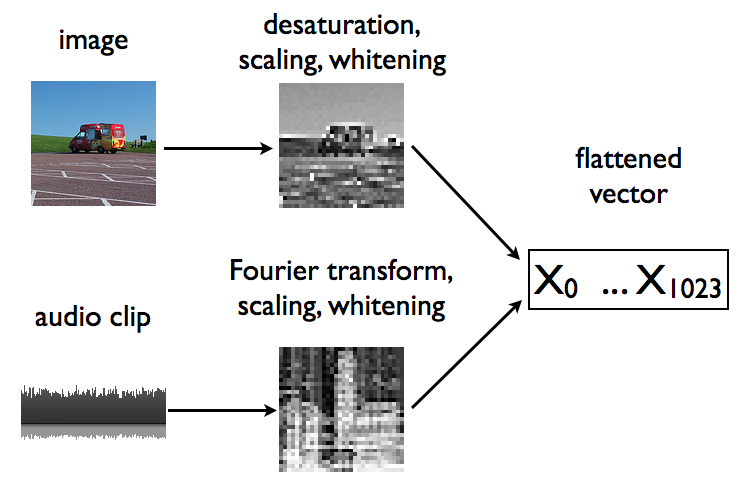
\includegraphics[width=6in]{key1002}
\caption{The data from both sensory modalities is preprocessed to create vectors of the same dimensionality to use as input to the learning algorithms.}
\end{figure}

\begin{figure}[p]
\centering
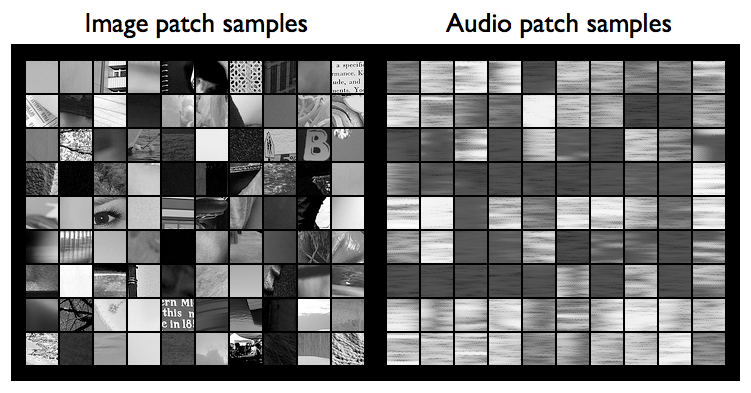
\includegraphics[width=6in]{patch_samples}
\caption{Patches sampled from the Flickr-1M dataset and spectrograms patches from the talk-show and radio broadcast dataset. These are the values prior to whitening.}
\label{fig:bothpatches}
\end{figure}
	
	To the best of my knowledge there is no comparably rich, large, and well packaged audio dataset released under Creative Commons or in the public domain, so for my experiments I am using a collection of publicly aired talk-show broadcasts from which short clips are sampled and transformed into spectrograms of comparable dimensions to the image patches. The patches of spectrogram are 500 milliseconds long, divided into 32 time bins. They are also divided into frequency bins of 32 peak frequencies on a logarithmic scale with the lowest frequency peak being 50 hz and the highest being 10 khz. An equal number of samples were prepared from each sensory modality, images and sounds, and each datum is of the same dimensionality, and is normalized in the same way. This way they can all be treated interchangeably, simplifying the code, and ensuring that any differences in learning between the two datasets are due to the differences in the content of their data, and not, for example, a different network topology for data of different dimensions.
	
\section{Results and Conclusion}
	\subsection{Experimental results}
	Hypothesis 1 is that networks pre-trained on one sensory modality performed better on the other modality than randomly initialized networks trained for an equal total number of epochs. To determine whether this has been confirmed I compare the reconstruction error from pairs of experiments where one was single-modal and the other was multi-modal, but the other variables were constant. There are four pairs: (1,2), (3,4), (5,6), and (7,8). The reconstruction errors are plotted in figure~\ref{fig:boxplots}. Cross modal initialization seems to have helped for models which were tested on audio, but actually hindered performance on models which were tested on images. For each pair in the figure, the second box plot (multi-modal models) is expected to lie completely to the left of it's single modal counterpart. The differences in means of the four pairs of experiments are tabulated in figure~\ref{fig:hypo1table}. 
	
\begin{figure}[p]
\centering
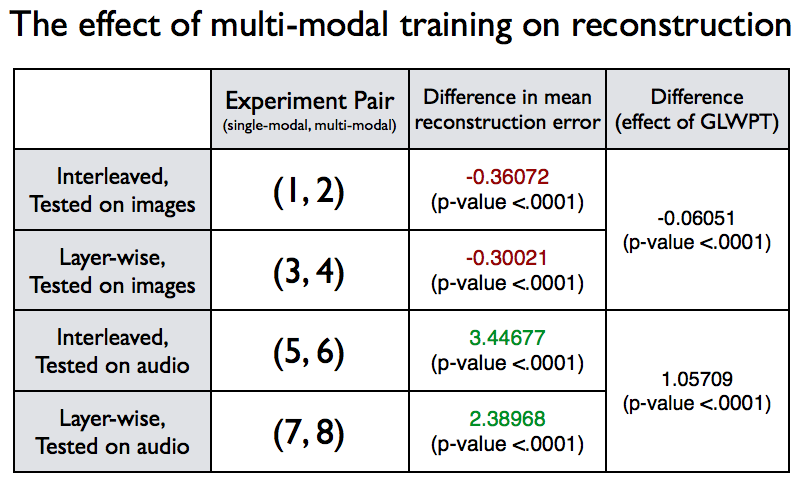
\includegraphics[width=6in]{hypo1table}
\caption{In this case when the difference in mean reconstruction error is positive, the multi-modal model performed better (lower reconstruction error). The column on the far right contains the differences in the difference in mean reconstruction error. Hypothesis 2 predicts that these will be negative. }
\label{fig:hypo1table}
\end{figure}

The second hypothesis is that the magnitude of improvement gained from cross-modal initialization is greater when GLWPT is applied than when it is not. I found that it was only improved for models tested on audio, and the size of the improvement was small. For models tested on audio (Experiments 5,6,7, and 8), layer-wise pre-training increased the improvement from cross-modal initialization, and in the case where cross-modal initialization hindered performance (Experiments 1,2,3 and 4) layer-wise pre-training lessened the amount it hindered.
	
\begin{figure}[p]
\centering
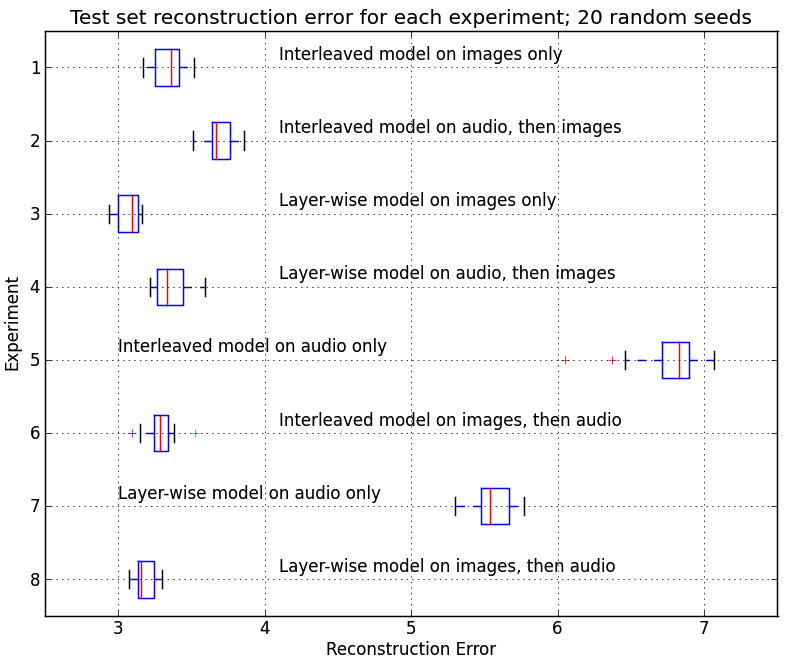
\includegraphics[width=6in]{boxplot}
\caption{Box plots of the reconstruction error for each of the 8 experiments. Lower reconstruction error means better performance. Interestingly, the single-modal audio models had relatively poor performance. Layer-wise pre-training helped somewhat, but multi-modal initialization helped much more.}
\label{fig:boxplots}
\end{figure}
	
\begin{figure}[p]
\centering
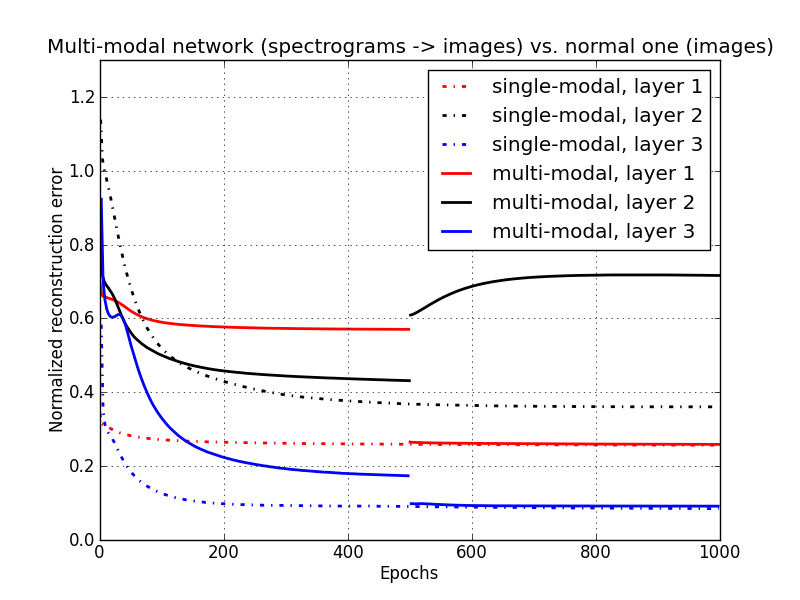
\includegraphics[width=6in]{graph_im_multi}
\caption{This graph compares a single interleaved network trained for 1000 epochs on images (dotted line) vs an interleaved network trained for 500 epochs on spectrograms, and then switched to images. Note the discrepancies between lines of the same color on the right half of the graph. The first and third layers see almost no change, but the second layer has two notable features. It begins in an unstable position, and then approaches a higher reconstruction error and stabilizes. This indicates that the structure of layer 1 is changing underneath it and altering it's fitness landscape, even which layer one's reconstruction error is stable.}
\label{fig:graph_im_multi}
\end{figure}

\begin{figure}[p]
\centering
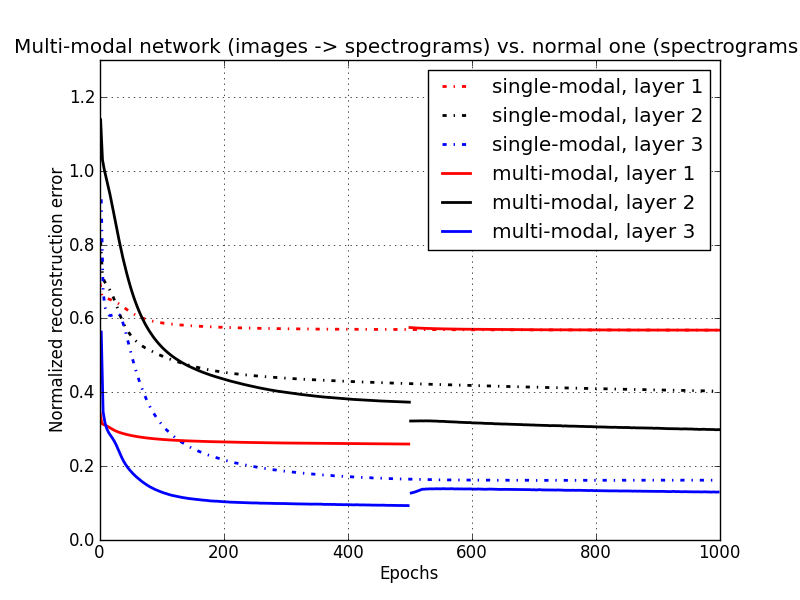
\includegraphics[width=6in]{graph_spect_multi}
\caption{This graph, similar to the one above, compares a single interleaved network trained for 1000 epochs on spectrograms (dotted line) vs an interleaved network trained for 500 epochs on images, and then switched to spectrograms. (the modalities are opposite) The strangest feature of this graph is that the reconstruction error for layers 2 and 3 on spectrograms is lower for the network trained on images than the one trained on spectrograms. This indicates that images make good training data, even if the test data is not images.}
\label{fig:graph_spect_multi}
\end{figure}
	
	In order to understand what is happening to the multi-modal networks at the point when the sensory modality is switched, I have graphed the normalized reconstruction error (reconstruction error divided by the number of nodes in the layer) for each layer in a pair of models. Figure~\ref{fig:graph_im_multi} shows the networks from experiments 1 and 2 (images), and figure~\ref{fig:graph_spect_multi} shows the networks from experiments 5 and 6 (audio). Layers are distinguished by colors, and the two networks are distinguished by line type.  Note what happens to each of the solid lines in the second phase of training in each graph, relative to the dotted line of the same color. The reconstruction error of each layer in the multi-modal model (solid line) is expected to start higher than the reconstruction error of the corresponding layer of the single-modal graph, and then slowly drop, hopefully below the dotted line of the same color, but this is not what happens at all. In the case of models tested on images (figure~\ref{fig:graph_im_multi}) layers one through three in the multi-modal model begin in a normal order, with lower normalized reconstruction error for the higher layers while it is training on spectrograms, but after the switch to images, layers 1 and 3 immediately begin at the same reconstruction error that layers 1 and 3 of the pure image network have already converged on, both quite lower. But strangely, the second layer's reconstruction error jumps above the 1st, and begins to increase significantly, Unfortunately I have no plausible explanation for this. 
	
	In the spectrogram experiment pair (figure~\ref{fig:graph_spect_multi}) There is a milder and reversed scenario. The pure-spectrogram network (dotted line) begins to converge with poor reconstruction error, just as it did in the multi-modal case in experiment 5, only this time it is left alone. Meanwhile the model being trained on images is converging to a lower reconstruction error with it's characteristic out-of-order layers. After the switch, the layers re-arrange to the order they are found in the spectrogram network, but with lower reconstruction error.
	
	When training any unsupervised learning algorithm, it is difficult to know whether the network has succeeded in learning the representations one expects. Measuring reconstruction error on test data gives an indication of how lossless the compression performed by the network is, but the goal is not perfectly lossless compression, it is generalizability and the discovery of interesting salient features that are useful to higher levels and similar networks. This is why it is crucial to visualize the features in the network. By working backwards from the weights, one can reconstruct an image that would maximally activate each node in a layer (figure ~\ref{fig:feature_comparison}). After performing this analysis on my networks, it seems that in all cases, about half of the nodes remain unused because they show no spatial correlation. The number of unused nodes is greater for audio than for images, and this may account for the significant differences between the results.

\begin{figure}[p]
\centering
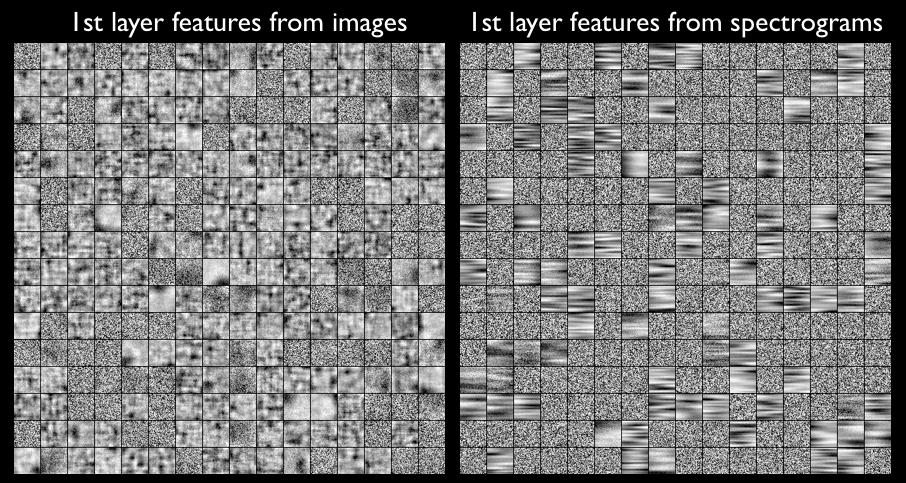
\includegraphics[width=6in]{feature_comparison}
\caption{These grids of feature detectors are created by working backwards from the weights in the first-level denoising autoencoder to obtain the image which would maximally activate each node. If we compare visual representations of the first level features of the pure image network and the pure spectrogram network, we see that there are two main differences. In the image network, more of the features converge on smooth edge and spot detectors, whereas in the spectrogram network, fewer of the features are utilized. Any feature resembling uniform noise is basically not being used. The other difference is that the spectrograms appear stretched, because their vertical axis is frequency and the horizontal axis is time, the scale of features on these axes could be adjusted to be more like the images if desired.}
\label{fig:feature_comparison}
\end{figure}
	

	
	\subsection{Conclusion and future work}
%In conclusion I found that GLWPT helped the SDAs learn abstract features, but this did not help it's cross-modal generalization. I address the unexpected differences between models tested on audio vs. images, and discuss potential causes and fixes. I include visualizations of the features learned and graphs of the reconstruction error over time for each layer in several pairs of models. These figures illustrate interesting unexpected observations about the training process which could be the focus of future work.
The results were unexpected because they did not exactly confirm or deny either hypothesis. The largest differences were between models tested on audio vs. models tested on images. The most interesting finding to me was that models trained on images, then audio performed far better when tested on audio than the models trained on only audio, but that this does not apply to models trained on audio first, then images, and tested on images. One interpretation of this finding is that a data driven pre-training step is the most helpful kind of regularizer, but that the data used for pre-training does not necessarily need to be from the same distribution as the data that the network is intended for. There may be a data-set that serves as a good pre-training set for a variety of problems. Demitru Erhan et al. have performed an experiment to rule out the possibility that the pre-training advantage could be explained simply by a better conditioning of the initial weights \cite{erhan2009difficulty}. They drew weights from the same range and marginal distribution as weights that were captured from a network already trained on data from the same dataset. They found that this offered an advantage over no layer-wise pre-training, but not as much as layer-wise pre-training using the actual dataset. They sampled weights from histograms of weights from a trained network but some of the useful data captured by the pre-training may have been lost in this process. I believe there may still be a possibility that a properly initialized network could have the same advantage of data-driven pre-training, and this would be an interesting topic of future work.

	In Figure~\ref{fig:bothpatches}, sample patches are arranged from both datasets. One can see that that there are several consistent differences. The image dataset contains a large number of high-contrast edges in a variety of angles and sizes. After whitening, the spectrograms will also become high-contrast, but they contain less high-contrast edges to begin with, and they are all flowing in the same direction and are relatively smooth. In figure~\ref{fig:feature_comparison} you can see visualizations of the features learned by the 1st layer of the image-only layer-wise denoising autoencoder and the audio-only layer-wise denoising autoencoder. Features in the audio network look more like data examples, while features in the image network are more general spot and edge detectors. In addition, there are more used features in the image network, while as many as 60\% of the features in the audio network remain unused. Why did the image dataset produce a better prior distribution? What statistical properties should we look for in good pre-training data? High information content would be my guess. If it doesn't compress well, it's probably going to be good for pre-training. Again, this would make an interesting topic for future work. The interesting layer-order anomaly shown in figure~\ref{fig:graph_spect_multi} also hints at a difference in the image dataset that may turn out to be characteristic of datasets which are good for pre-training. The second layer has a higher reconstruction error in that model, whereas in other models, the normalized reconstruction errors are in layer order.
	
	In the introduction, I discussed the motivation for studying plasticity because it gives us an idea of how brain-like the SDA algorithm is. If intelligence is too difficult to measure or to difficult to achieve, then maybe esoteric behaviors and qualities of the brain will be more helpful indicators. It would be very interesting to look for this sensory imbalance in animal or human studies of neuroplasiiicity. Does the primary visual cortex adapt more quickly or effectively to auditory stimulation than the auditory cortex can adapt to visual stimulation? There have been studies of both instances of neuro-plasticity \cite{ryugo1975increased, gyllensten1966growth}, but no direct comparisons as far as I know. 
	
	In conclusion, these experiments may re-open the question of whether properly initialized data-agnostic weights can offer the same benefit of data-driven pre-training. Pre-training adds robustness to a deep architecture, but it may not be the most effective or fastest way to add robustness. A hierarchical structure alone is not sufficient to allow plasticity and adaptability, nor is it even a matter of training method, but a matter of the weights. SDA's are not a magic bullet for discovering abstract features, but they are one of the best algorithms available at the current time. A more careful tuning of hyper-parameters, and a broader exploration of pre-training data sources would lead to further discoveries on the path to matching the power and adaptability of the neocortex.

\end{doublespacing}

\singlespacing
\bibliographystyle{plain}
\bibliography{machine_learning_bibliography}


% figures are inturrupting the bibliography! fix it.

\end{document}






